\documentclass[11pt,a4paper]{article}

\usepackage{../style/thga-db}
\usepackage{caption}
\usepackage{float}
\usepackage{tikz}
\usetikzlibrary{arrows.meta,positioning}

\renewcommand{\thgaKurs}{Databases}
\renewcommand{\thgaDatum}{Summer Term 2026}
\newcommand{\authorName}{Mohamed Yassine Hachimi}
\newcommand{\projectTitle}{HandwerkerKasse -- Developer Documentation}

\begin{document}
\thispagestyle{empty}
\thgaTitel{Term Project -- Developer Documentation}{\projectTitle}

\begin{infobox}
\textbf{Author:} \authorName \\
\textbf{Module:} Introduction to Database Management Systems · THGA Bochum \\
\textbf{Audience:} developers who want to run, test, extend, or deploy the system.
\end{infobox}

\section{Architecture overview}

HandwerkerKasse follows a three-tier architecture: a Tkinter desktop frontend communicates over HTTP with a FastAPI backend, which in turn talks to a PostgreSQL database. Write operations require a valid X-API-Key header; read operations are open.

\begin{center}
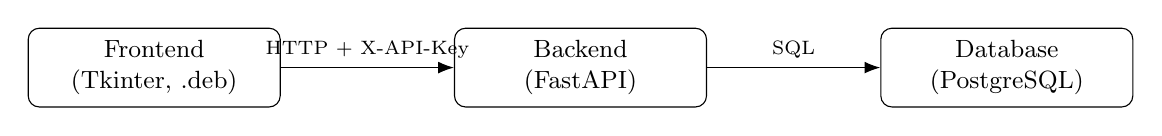
\begin{tikzpicture}[
  box/.style={draw, rounded corners, minimum width=3.2cm, minimum height=1cm, align=center, font=\small},
  node distance=2.2cm
]
  \node[box] (frontend) {Frontend\\(Tkinter, .deb)};
  \node[box, right=of frontend] (backend) {Backend\\(FastAPI)};
  \node[box, right=of backend] (db) {Database\\(PostgreSQL)};

  \draw[-{Latex[length=2mm]}] (frontend) -- node[above,font=\scriptsize]{HTTP + X-API-Key} (backend);
  \draw[-{Latex[length=2mm]}] (backend) -- node[above,font=\scriptsize]{SQL} (db);
\end{tikzpicture}
\end{center}

Both the backend and the database run as containers, orchestrated with Docker Compose. The frontend is installed separately as a Debian package on the client machine.

\section{Database schema}

The database consists of five tables: \texttt{customers}, \texttt{jobs}, \texttt{materials}, \texttt{job\_materials} and \texttt{invoices}. The schema follows the third normal form (3NF); every table stores one type of information, and relationships are expressed through foreign keys.

\begin{verbatim}
CREATE TABLE customers (
    id         SERIAL PRIMARY KEY,
    name       VARCHAR(150) NOT NULL,
    email      VARCHAR(150),
    phone      VARCHAR(50)
);

CREATE TABLE jobs (
    id          SERIAL PRIMARY KEY,
    customer_id INTEGER NOT NULL REFERENCES customers(id) ON DELETE CASCADE,
    title       VARCHAR(200) NOT NULL,
    status      VARCHAR(50) NOT NULL DEFAULT 'open'
                CHECK (status IN ('open','in_progress','completed','cancelled')),
    job_date    DATE NOT NULL DEFAULT CURRENT_DATE
);

CREATE TABLE materials (
    id             SERIAL PRIMARY KEY,
    name           VARCHAR(150) NOT NULL,
    purchase_price NUMERIC(10,2) NOT NULL CHECK (purchase_price >= 0)
);

CREATE TABLE job_materials (
    id          SERIAL PRIMARY KEY,
    job_id      INTEGER NOT NULL REFERENCES jobs(id) ON DELETE CASCADE,
    material_id INTEGER NOT NULL REFERENCES materials(id) ON DELETE RESTRICT,
    quantity    NUMERIC(10,2) NOT NULL CHECK (quantity > 0),
    UNIQUE (job_id, material_id)
);

CREATE TABLE invoices (
    id             SERIAL PRIMARY KEY,
    job_id         INTEGER NOT NULL UNIQUE REFERENCES jobs(id) ON DELETE CASCADE,
    amount         NUMERIC(10,2) NOT NULL CHECK (amount >= 0),
    payment_status VARCHAR(50) NOT NULL DEFAULT 'unpaid'
                   CHECK (payment_status IN ('unpaid','paid','overdue'))
);
\end{verbatim}

Figure~\ref{fig:seed} shows the database populated with seed data, queried directly via \texttt{psql}. Figure~\ref{fig:container} shows the PostgreSQL container running in a healthy state.

\begin{figure}[H]
  \centering
  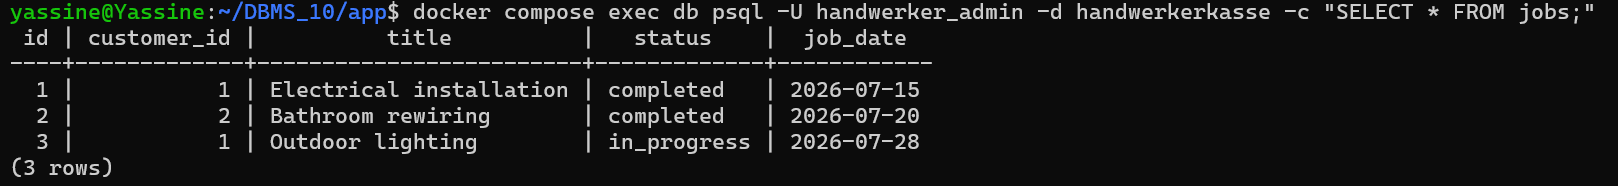
\includegraphics[width=0.85\linewidth]{01_db_seed-data-jobs.png}
  \caption{Seed data loaded into the jobs table}
  \label{fig:seed}
\end{figure}

\begin{figure}[H]
  \centering
  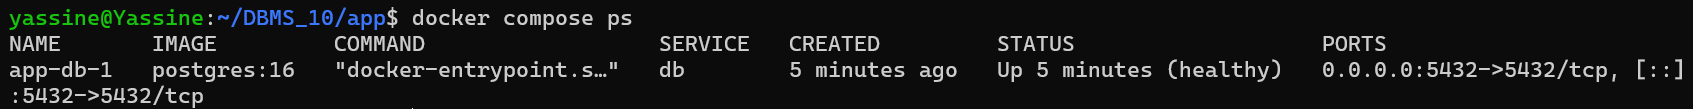
\includegraphics[width=0.85\linewidth]{02_db_container-running.png}
  \caption{PostgreSQL container running and healthy}
  \label{fig:container}
\end{figure}

\section{API reference}

The FastAPI backend exposes the following endpoints. All write operations (POST, PUT, DELETE) require a valid \texttt{X-API-Key} header; read operations (GET) are open.

\renewcommand{\arraystretch}{1.2}
\begin{tabularx}{\linewidth}{@{}p{2cm}p{4cm}X@{}}
\toprule
\textbf{Method} & \textbf{Path} & \textbf{Purpose} \\
\midrule
\texttt{GET} & \texttt{/customers} & Returns all customers. \\
\texttt{POST} & \texttt{/customers} & Creates a new customer. Requires X-API-Key. \\
\texttt{GET} & \texttt{/jobs} & Returns all jobs. \\
\texttt{POST} & \texttt{/jobs} & Creates a new job. Requires X-API-Key. \\
\texttt{PUT} & \texttt{/jobs/\{id\}} & Updates an existing job. Requires X-API-Key. \\
\texttt{DELETE} & \texttt{/jobs/\{id\}} & Deletes an existing job. Requires X-API-Key. \\
\texttt{GET} & \texttt{/materials} & Returns all materials. \\
\texttt{POST} & \texttt{/materials} & Creates a new material. Requires X-API-Key. \\
\texttt{POST} & \texttt{/job\_materials} & Assigns a material and quantity to a job. Requires X-API-Key. \\
\texttt{GET} & \texttt{/invoices} & Returns all invoices. \\
\texttt{POST} & \texttt{/invoices} & Creates a new invoice. Requires X-API-Key. \\
\texttt{GET} & \texttt{/jobs/profit} & Returns jobs with calculated profit values. \\
\bottomrule
\end{tabularx}

Figure~\ref{fig:swagger} shows the interactive API documentation, automatically generated by FastAPI and available at \texttt{/docs} on the running server.

\begin{figure}[H]
  \centering
  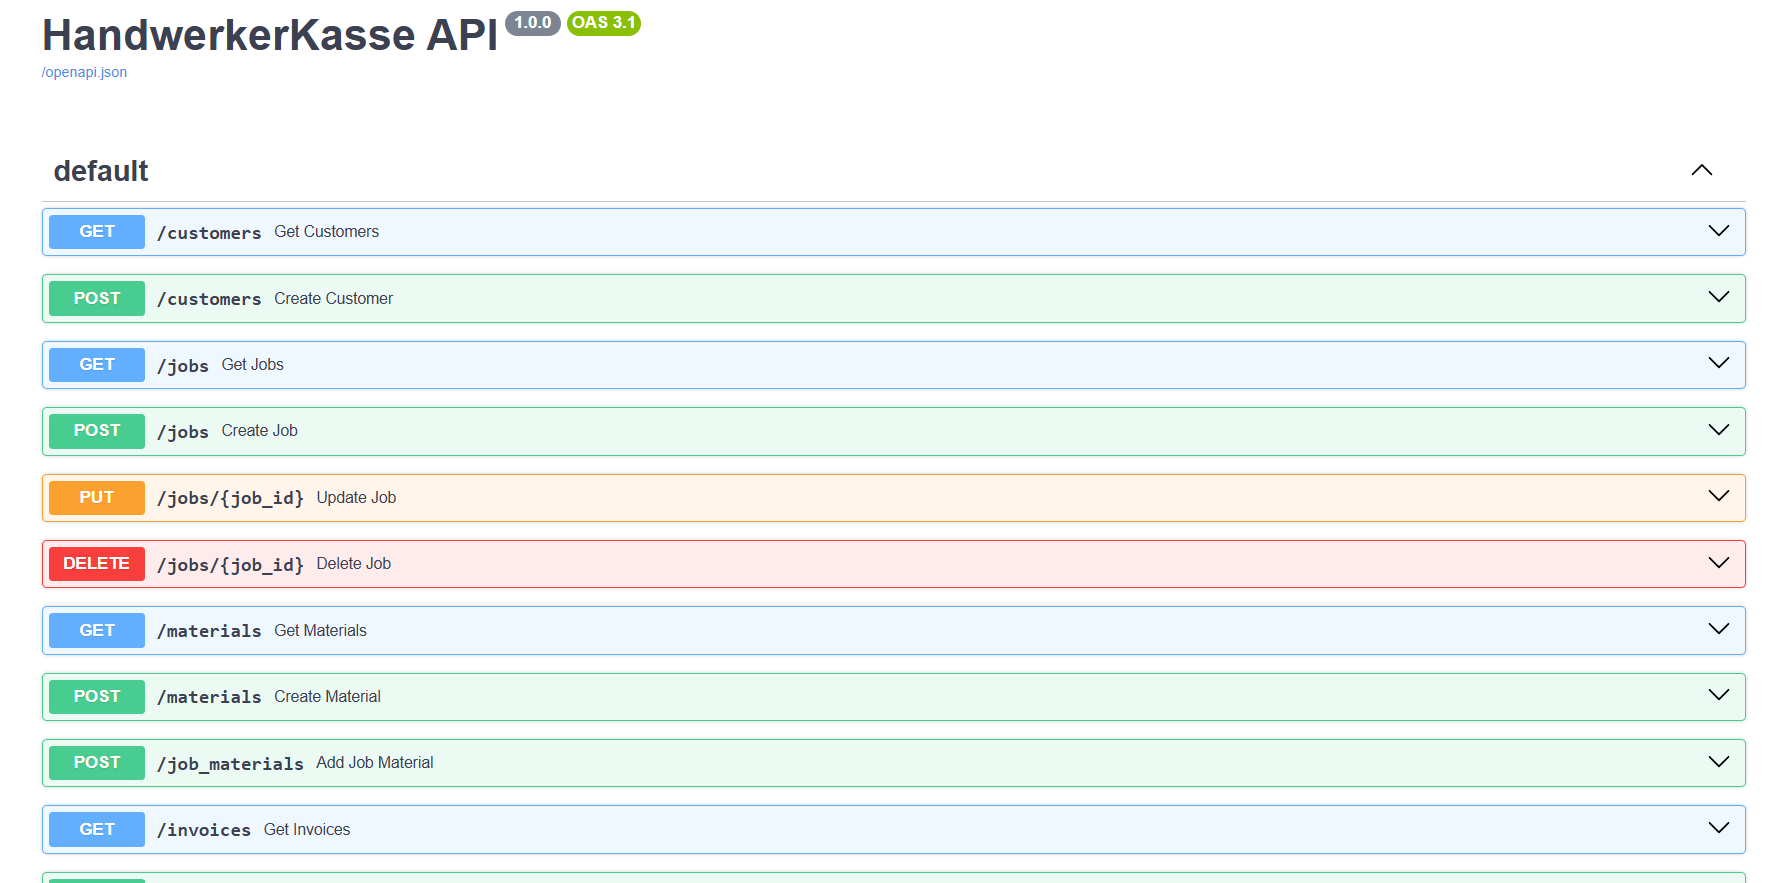
\includegraphics[width=0.9\linewidth]{03_api_swagger-overview.png}
  \caption{Automatically generated Swagger UI listing all endpoints}
  \label{fig:swagger}
\end{figure}

\subsection{Profit calculation}

The endpoint \texttt{GET /jobs/profit} is the core feature of the system. It joins \texttt{jobs}, \texttt{invoices}, \texttt{job\_materials} and \texttt{materials}, aggregates the material cost per job, and returns:

\[
\text{Profit} = \text{Invoice Amount} - \sum(\text{Quantity} \times \text{Purchase Price})
\]

Figure~\ref{fig:profit} shows a live response from this endpoint, confirming the calculation works correctly against real data.

\begin{figure}[H]
  \centering
  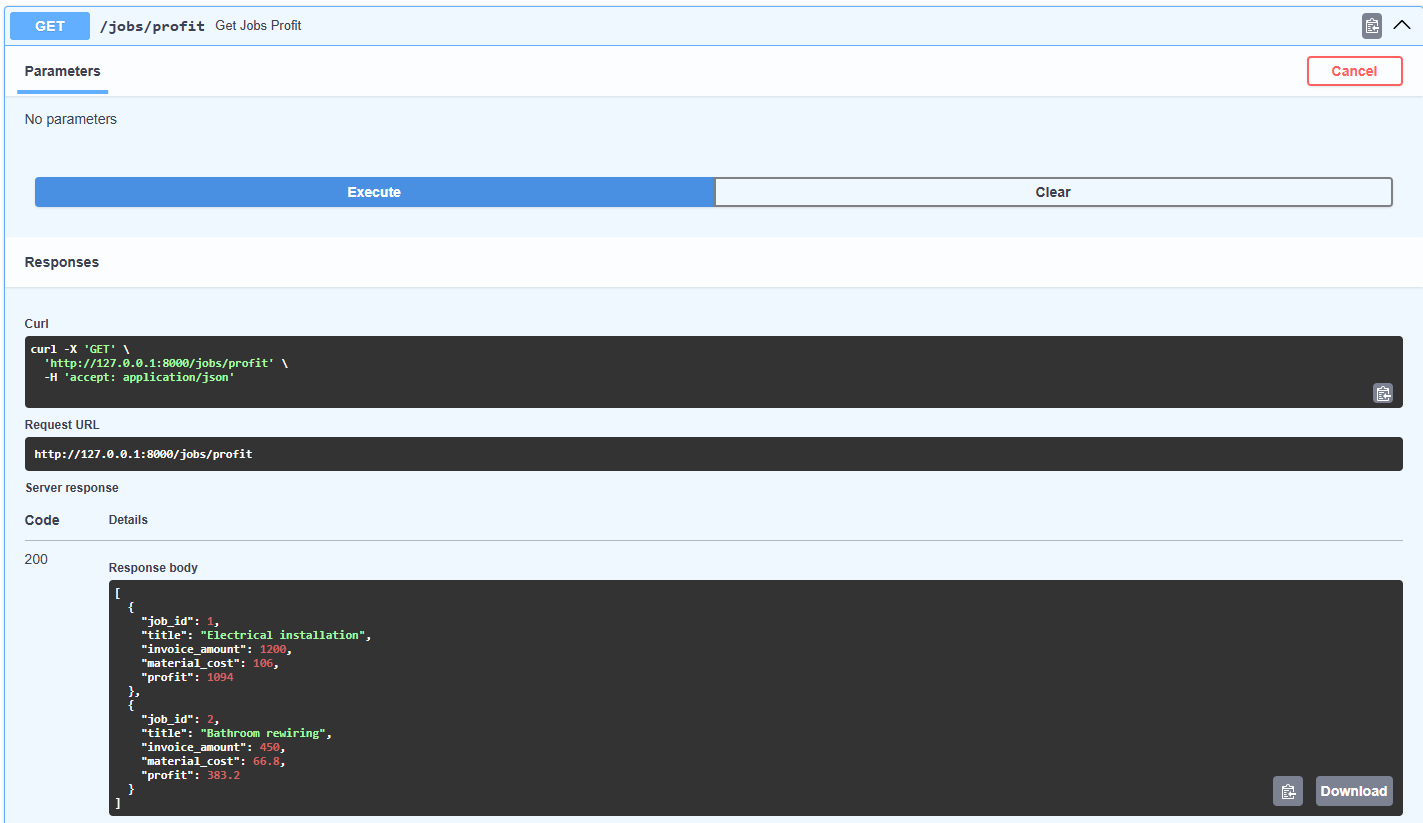
\includegraphics[width=0.9\linewidth]{05_api_jobs-profit-response_1.png}
  \caption{Live response of GET /jobs/profit}
  \label{fig:profit}
\end{figure}

\begin{figure}[H]
  \centering
  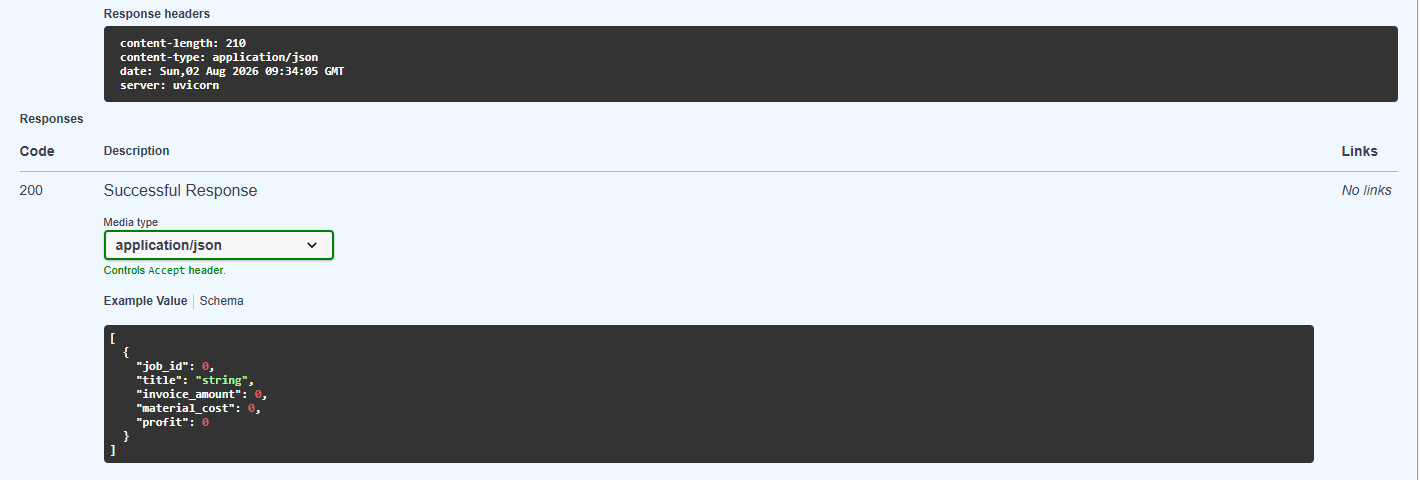
\includegraphics[width=0.9\linewidth]{05_api_jobs-profit-response_2.png}
  \caption{Live response of GET /jobs/profit (continued)}
  \label{fig:profit2}
\end{figure}

\subsection{Authentication}

Write endpoints reject requests without a valid \texttt{X-API-Key} with HTTP 401. Figure~\ref{fig:unauthorized} shows a rejected request, and Figure~\ref{fig:authorized} shows the same request succeeding once the correct key is provided.

\begin{figure}[H]
  \centering
  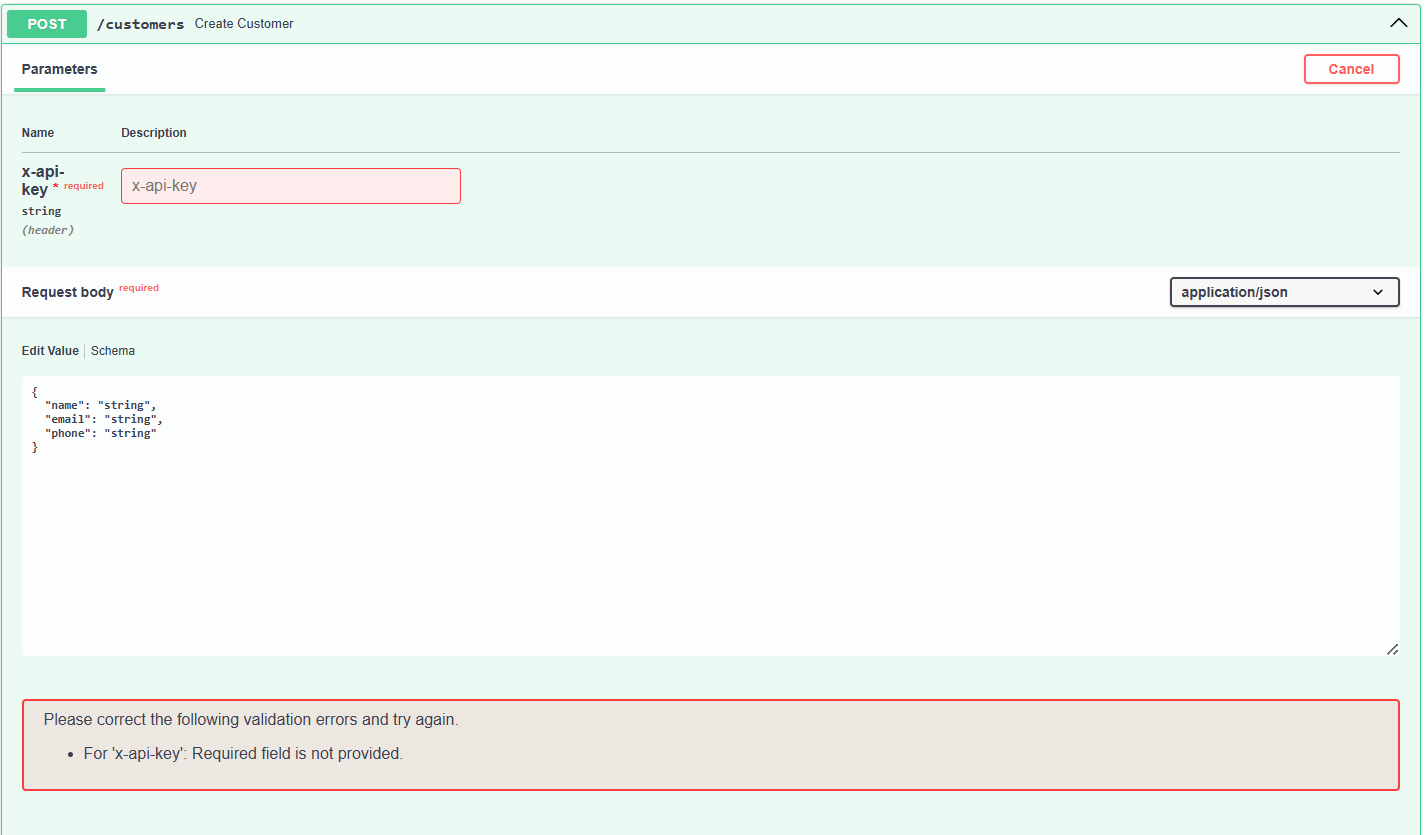
\includegraphics[width=0.9\linewidth]{06_api_post-customer-unauthorized.png}
  \caption{POST /customers rejected without a valid X-API-Key}
  \label{fig:unauthorized}
\end{figure}

\begin{figure}[H]
  \centering
  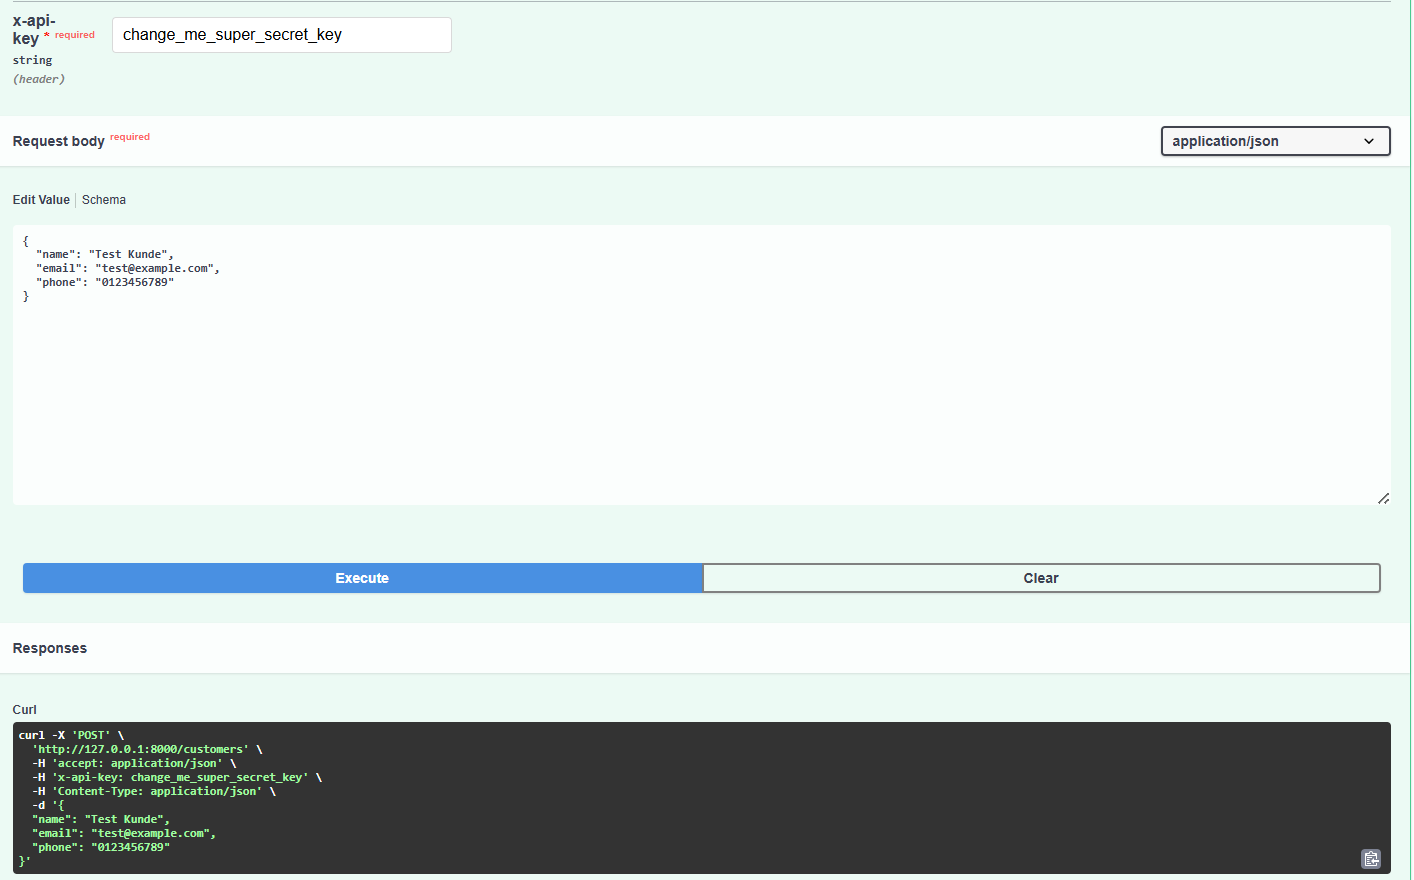
\includegraphics[width=0.9\linewidth]{07_api_post-customer-success_1.png}
  \caption{POST /customers succeeding with a valid X-API-Key}
  \label{fig:authorized}
\end{figure}

\begin{figure}[H]
  \centering
  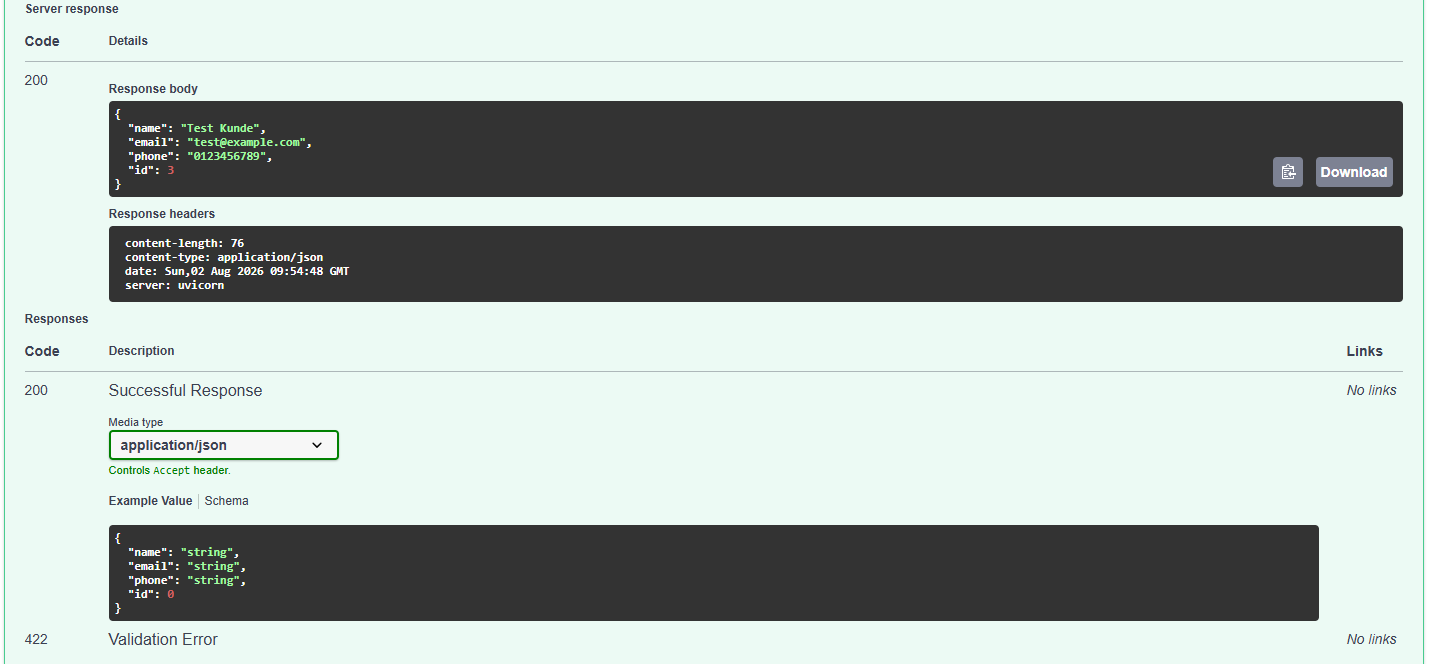
\includegraphics[width=0.9\linewidth]{07_api_post-customer-success_2.png}
  \caption{POST /customers response body showing the created customer}
  \label{fig:authorized2}
\end{figure}

\subsection{Reading data}

Figures~\ref{fig:customers1} and~\ref{fig:customers2} show a full request/response cycle for \texttt{GET /customers}, confirming that seeded data is returned correctly as JSON.

\begin{figure}[H]
  \centering
  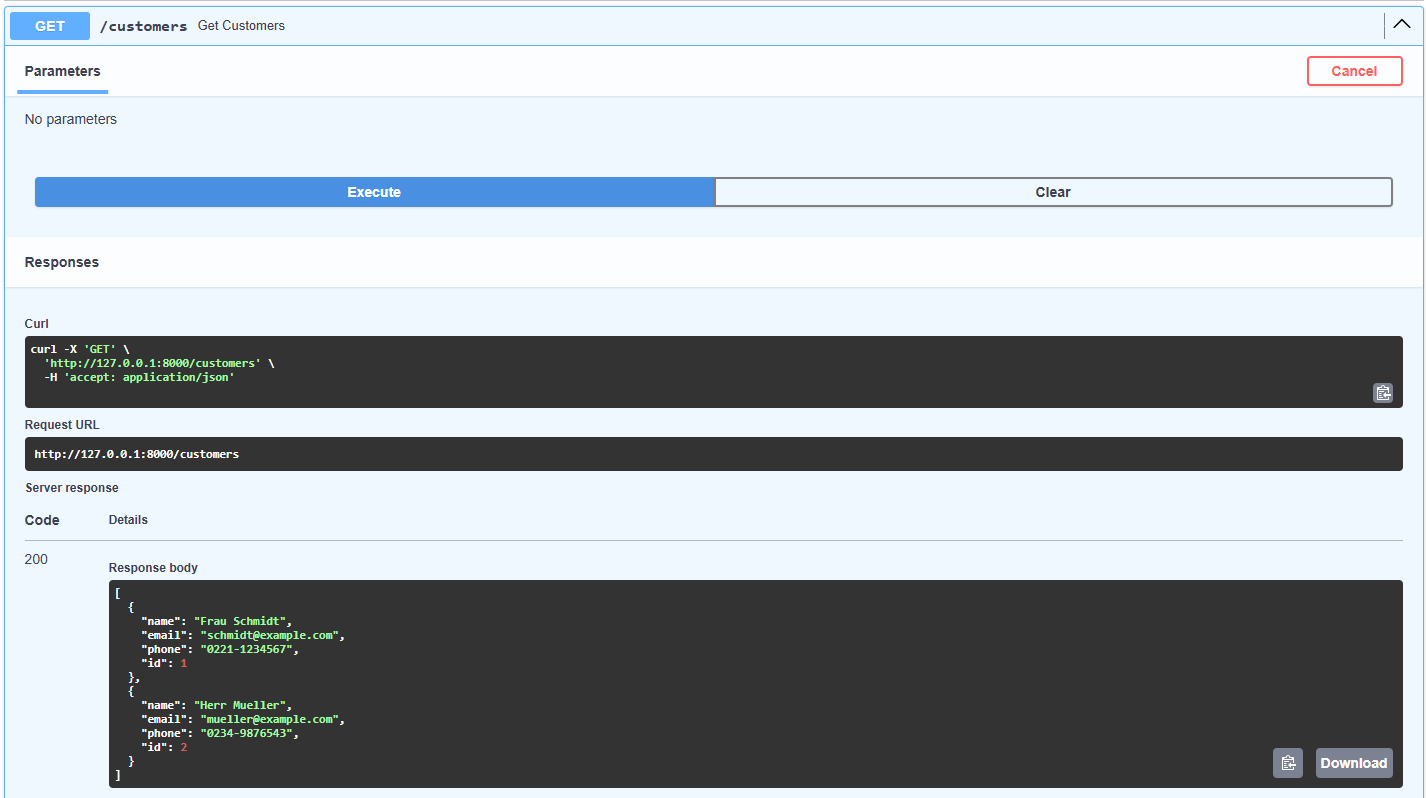
\includegraphics[width=0.9\linewidth]{04_api_get-customers-response_1.png}
  \caption{GET /customers request in Swagger UI}
  \label{fig:customers1}
\end{figure}

\begin{figure}[H]
  \centering
  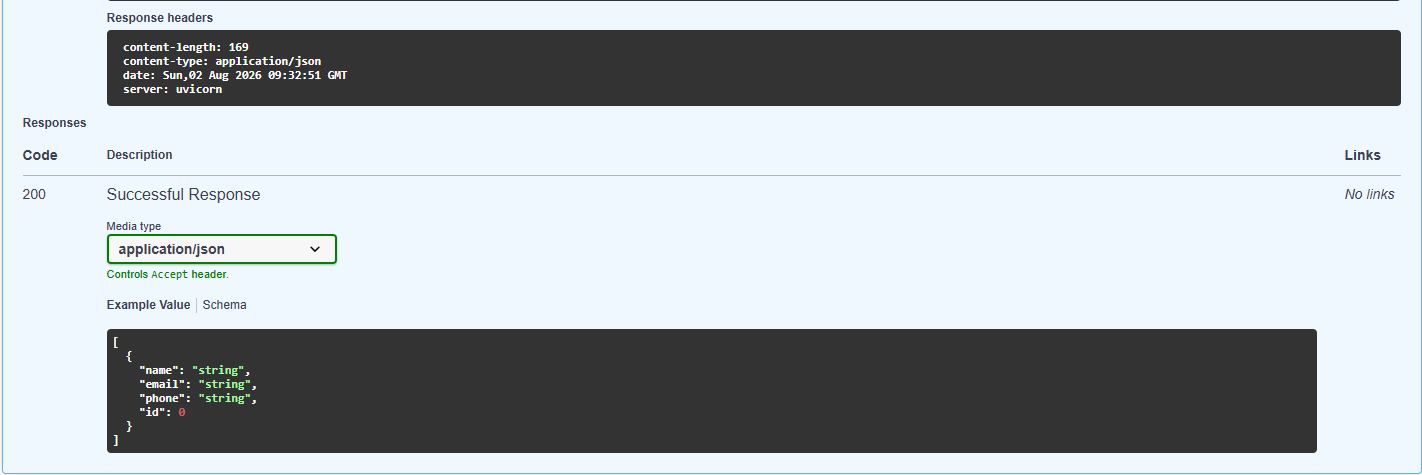
\includegraphics[width=0.9\linewidth]{04_api_get-customers-response_2.png}
  \caption{GET /customers response body}
  \label{fig:customers2}
\end{figure}

\section{Local development setup}

To run the backend locally without Docker:

\begin{verbatim}
cd app/backend
python3 -m venv venv
source venv/bin/activate
pip install -r requirements.txt
uvicorn main:app --reload
\end{verbatim}

The backend expects a \texttt{.env} file (in \texttt{app/}) with the following variables:

\begin{verbatim}
POSTGRES_USER=...
POSTGRES_PASSWORD=...
POSTGRES_DB=...
POSTGRES_PORT=5432
API_KEY=...
\end{verbatim}

\subsection{Project structure}

\begin{verbatim}
app/
  docker-compose.yml
  .env
  db/
    schema.sql
    seed.sql
  backend/
    Dockerfile
    main.py
    database.py
    models.py
    schemas.py
    requirements.txt
    conftest.py
    test_api.py
  frontend/
    api.py
    ui.py
    connection_dialog.py
    __main__.py
    requirements.txt
packaging/
  handwerkerkasse/
    DEBIAN/control
    opt/handwerkerkasse/main.py
    usr/bin/handwerkerkasse
    usr/share/applications/handwerkerkasse.desktop
\end{verbatim}

\section{Testing}

The backend is covered by an automated pytest suite (\texttt{test\_api.py}), using FastAPI's \texttt{TestClient} against an isolated test database. Tests cover the happy path, authentication failures, invalid foreign keys, and a full end-to-end scenario verifying the profit calculation.

\begin{verbatim}
cd app/backend
source venv/bin/activate
pytest -v
\end{verbatim}

Figure~\ref{fig:pytest} shows a full test run, confirming that all acceptance criteria defined in the proposal are met.

\begin{figure}[H]
  \centering
  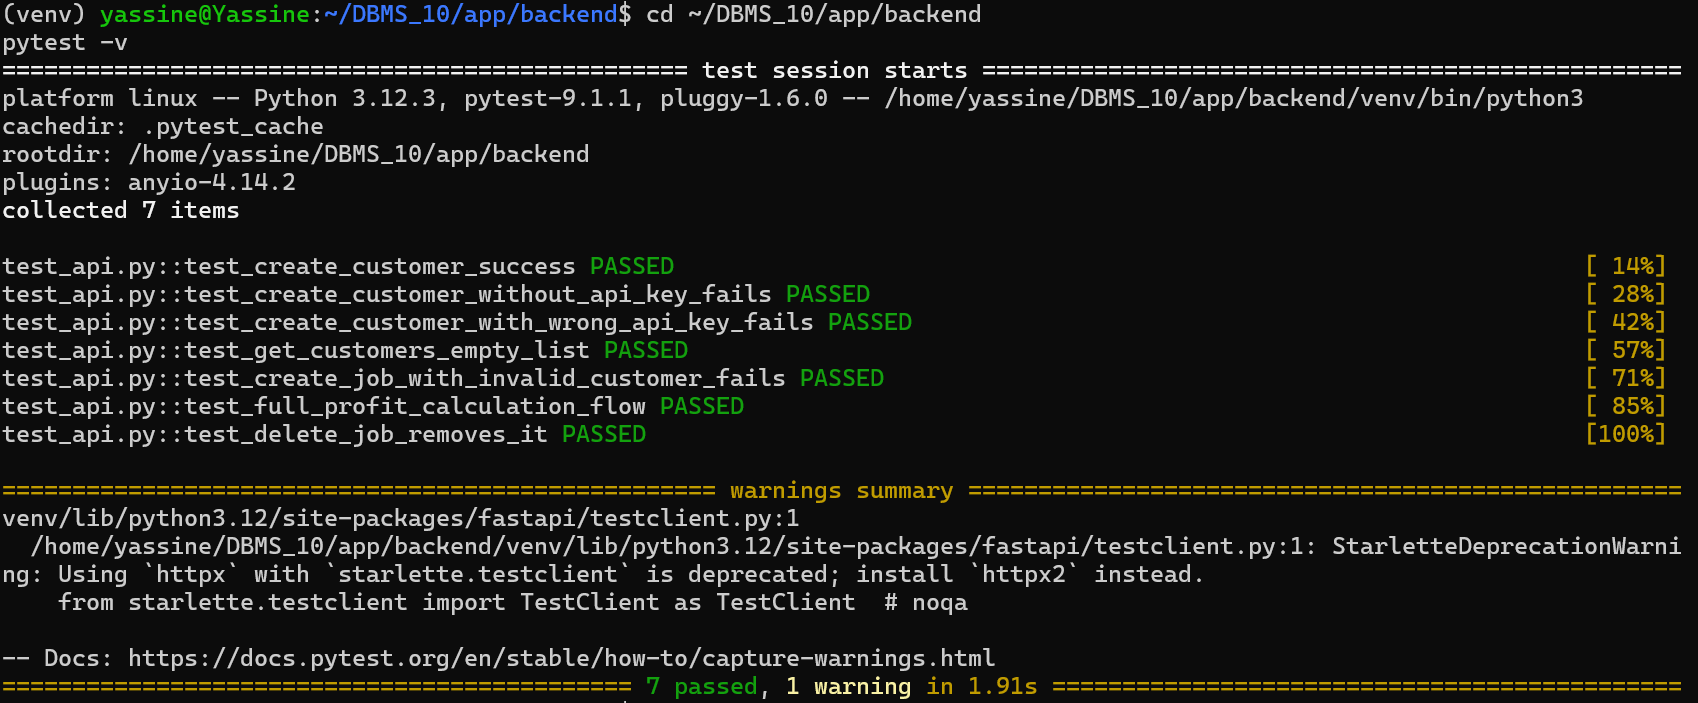
\includegraphics[width=0.9\linewidth]{08_test_pytest-passing.png}
  \caption{All automated tests passing}
  \label{fig:pytest}
\end{figure}

\section{Deployment with Docker Compose}

The backend and database are deployed together using Docker Compose. From the \texttt{app/} directory:

\begin{verbatim}
docker compose up -d --build
\end{verbatim}

This builds the backend image, starts PostgreSQL, waits for its health check, then starts the backend container connected to it via the internal Docker network (service name \texttt{db}). Figure~\ref{fig:compose} shows both containers running.

\begin{figure}[H]
  \centering
  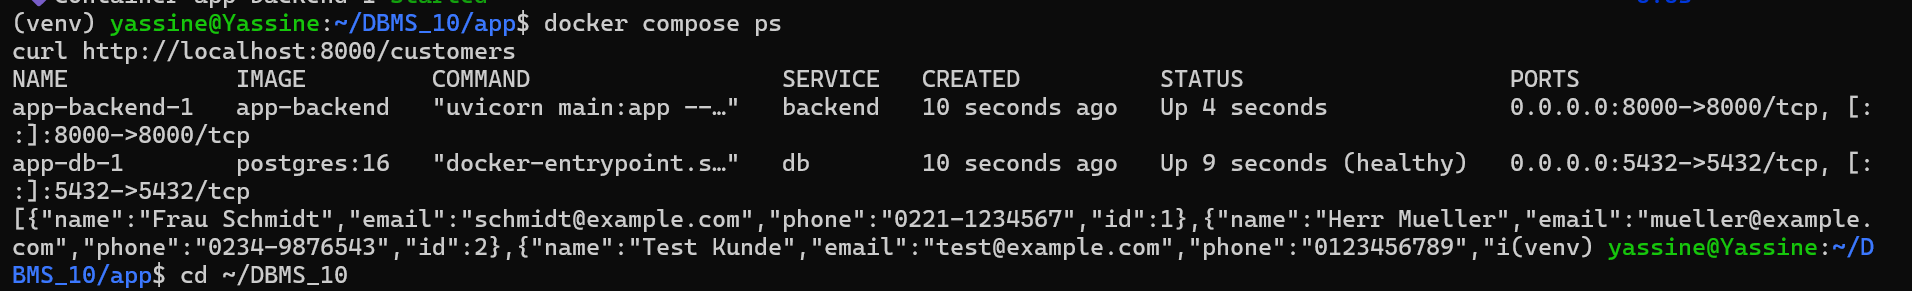
\includegraphics[width=0.9\linewidth]{13_deploy_docker-compose-both-running.png}
  \caption{Database and backend containers running together}
  \label{fig:compose}
\end{figure}

\section{Building and installing the frontend package}

The frontend is packaged as a Debian package for easy installation on client machines. The package structure is built manually and assembled with \texttt{dpkg-deb}:

\begin{verbatim}
cd packaging
dpkg-deb --build --root-owner-group handwerkerkasse
sudo apt install ./handwerkerkasse.deb
\end{verbatim}

Once installed, the application can be launched from the applications menu or via the \texttt{handwerkerkasse} command. Figure~\ref{fig:deb} shows the installed application running.

\begin{figure}[H]
  \centering
  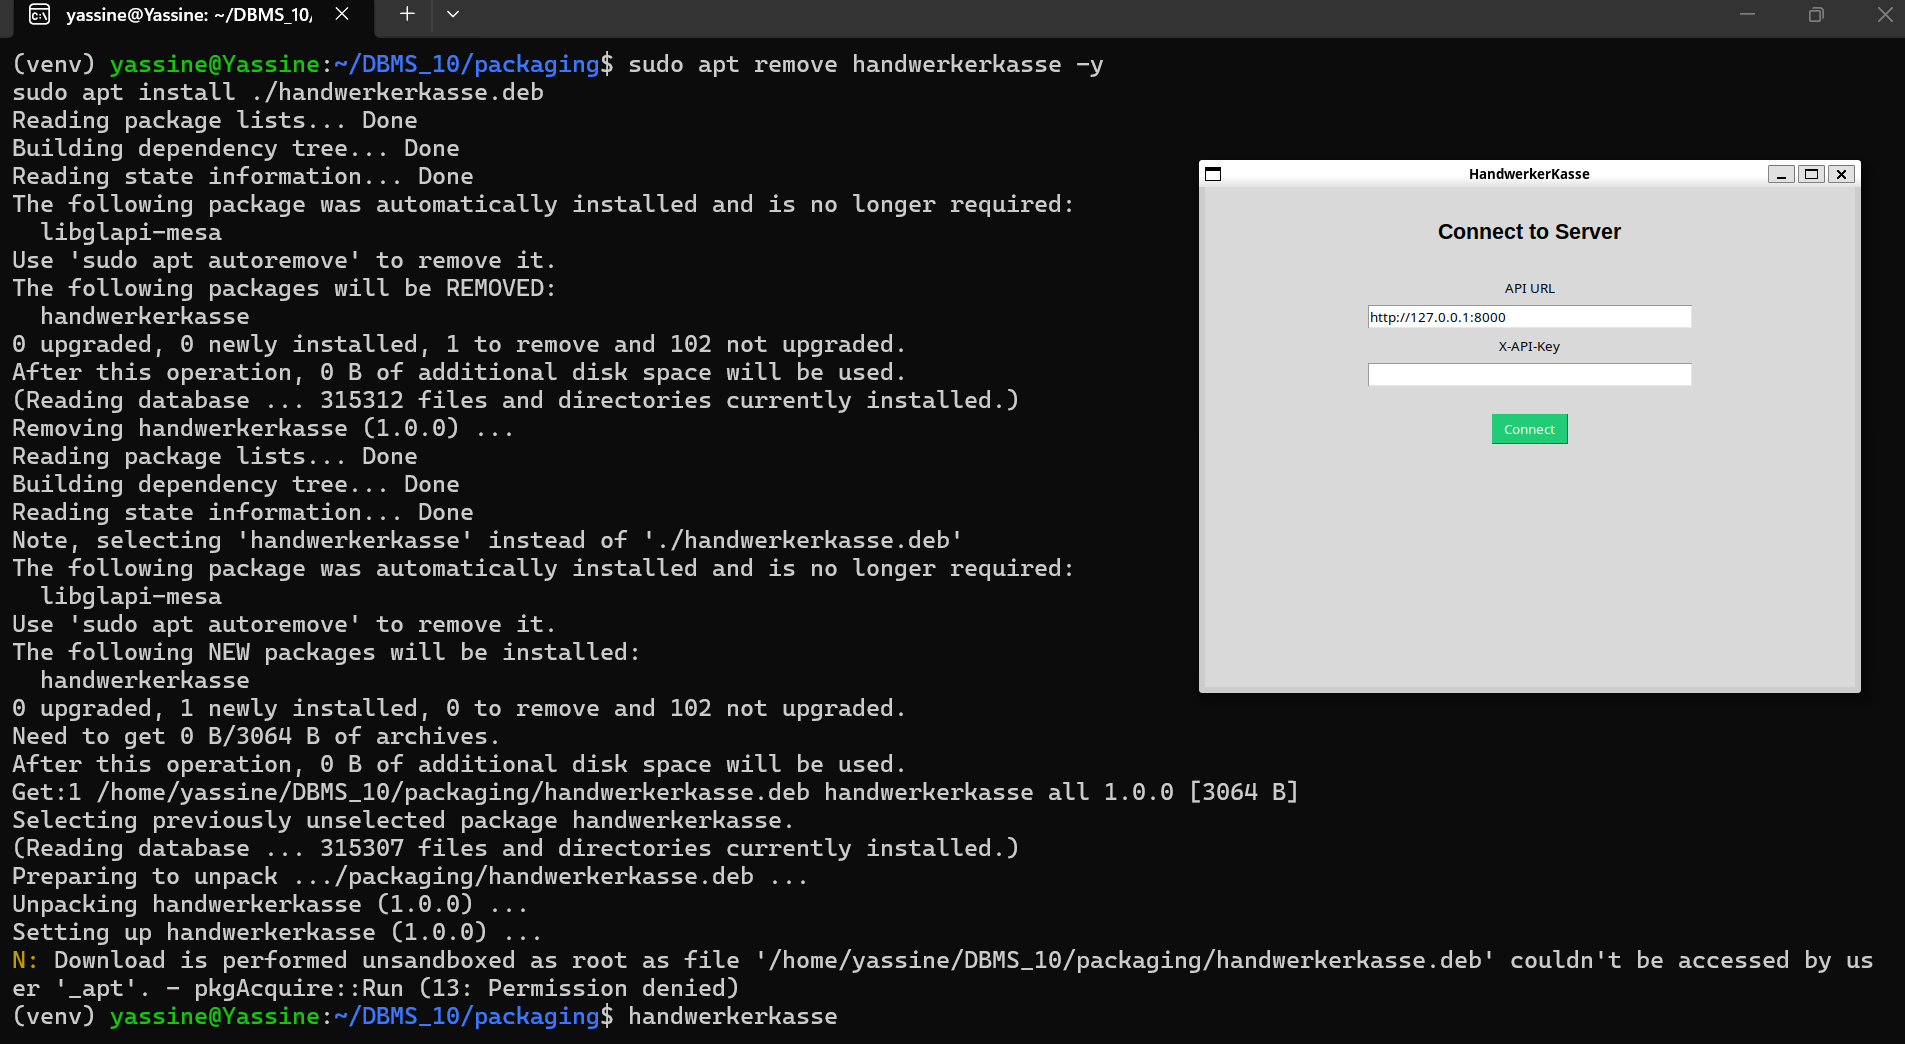
\includegraphics[width=0.6\linewidth]{14_deploy_deb-package-installed-running.png}
  \caption{Installed .deb package running as a desktop application}
  \label{fig:deb}
\end{figure}

\section{Extending the system}

The schema and API are designed to be extended without breaking existing functionality:

\begin{itemize}
  \item New fields can be added to existing tables with \texttt{ALTER TABLE}, keeping foreign key relationships intact.
  \item New endpoints follow the same pattern: a Pydantic schema in \texttt{schemas.py}, a SQLAlchemy model in \texttt{models.py} if needed, and a route in \texttt{main.py} using the \texttt{verify\_api\_key} dependency for write access.
  \item Possible extensions include inventory tracking for materials, multi-user support, or a dedicated endpoint for updating and deleting job-material assignments.
\end{itemize}

\section{Design decisions and how to modify them}

This section explains the reasoning behind key implementation choices, which parts of the system are optional or interchangeable, and how a developer would go about changing them.

\subsection{ORM vs. raw SQL (optional choice)}

The backend uses \textbf{SQLAlchemy} as an ORM instead of writing raw SQL queries directly with \texttt{psycopg2}. This was a deliberate but optional choice:

\begin{itemize}
  \item Each database table is represented as a Python class in \texttt{models.py} (e.g. \texttt{class Job(Base)}), with columns defined as class attributes and relationships declared explicitly (e.g. \texttt{relationship("Customer", back\_populates="jobs")}).
  \item This makes queries readable in Python (\texttt{db.query(models.Job).filter(...)}) instead of embedding SQL strings throughout the code, and it automatically handles foreign key joins through the declared relationships.
  \item \textbf{To switch to raw SQL:} replace the SQLAlchemy query calls in \texttt{main.py} with \texttt{psycopg2} cursor calls (already installed as a dependency, since SQLAlchemy uses it internally as the database driver). The database schema itself (\texttt{db/schema.sql}) would not need to change, since it is plain SQL independent of the ORM.
\end{itemize}

\subsection{Pydantic schemas (required, but extensible)}

Every endpoint uses a Pydantic model from \texttt{schemas.py} to validate incoming data (e.g. \texttt{CustomerCreate}) and to shape outgoing responses (e.g. \texttt{CustomerOut}). This is not optional -- FastAPI relies on these schemas for automatic request validation and for generating the Swagger documentation seen in Figure~\ref{fig:swagger}.

\textbf{To add a new field} (e.g. a \texttt{notes} field on jobs): add the column in \texttt{db/schema.sql}, add the attribute to the \texttt{Job} class in \texttt{models.py}, and add it to \texttt{JobCreate} and \texttt{JobOut} in \texttt{schemas.py}. No changes to \texttt{main.py} are needed, since the existing endpoints already forward all fields via \texttt{model\_dump()}.

\subsection{Authentication (optional to extend)}

Authentication is currently a single shared \texttt{X-API-Key}, checked by the \texttt{verify\_api\_key} dependency in \texttt{main.py}, applied per-endpoint via \texttt{dependencies=[Depends(verify\_api\_key)]}. This was a deliberate simplification for the project's scope (no user accounts, as agreed in the proposal).

\textbf{To extend this} to per-user authentication: a \texttt{users} table could be added, \texttt{verify\_api\_key} replaced with a function that validates a JWT or session token instead of a static string, and the dependency reused unchanged on all write endpoints, since the endpoint logic itself does not need to know how authentication is implemented.

\subsection{Frontend framework (optional choice)}

The frontend uses Python's built-in \texttt{tkinter} library rather than a more feature-rich framework such as PyQt. This was chosen for simplicity and easy \texttt{.deb} packaging, since \texttt{tkinter} ships with Python and requires no additional system libraries beyond \texttt{python3-tk}.

\textbf{To replace the frontend entirely:} any client capable of sending HTTP requests with an \texttt{X-API-Key} header can be used instead, since the frontend and backend are fully decoupled and communicate only over the documented REST API. A web frontend, a mobile app, or a different desktop framework could all be substituted without changing the backend.

\subsection{Docker Compose networking (fixed requirement)}

Unlike the previous points, the way the backend locates the database is \textbf{not} optional: the backend connects to the database using the Docker Compose service name (\texttt{db}) as the hostname rather than \texttt{localhost}, since containers on the same Compose network resolve each other by service name. This is controlled by the \texttt{DB\_HOST} environment variable, set to \texttt{db} in \texttt{docker-compose.yml} and defaulting to \texttt{localhost} for local development outside Docker (see \texttt{database.py}).

\subsection{Summary of extension points}

\begin{itemize}
  \item \textbf{Easy to change:} frontend framework, authentication mechanism, ORM vs. raw SQL.
  \item \textbf{Easy to extend without breaking anything:} new fields, new tables, new endpoints following the existing pattern.
  \item \textbf{Fixed by the deployment architecture:} the Docker Compose service name as the database host, and the REST/JSON contract between frontend and backend.
\end{itemize}

\section{Reflection questions}

This section answers the kind of conceptual questions a developer new to the project might ask, in the style used throughout this module.

\subsection*{Question: Why separate the API client logic from the UI code?}

In the frontend, all HTTP communication happens through simple function-style calls inside each screen class (e.g. \texttt{requests.post(...)} in \texttt{JobFormScreen.save\_job()}), rather than being scattered across the whole application. This keeps each screen responsible only for collecting input and displaying results, while the actual request format (headers, JSON body, error handling) stays consistent. If the API changed its authentication method, only these call sites would need updating, not the widget layout.

\subsection*{Question: Why does the backend use dependency injection (\texttt{Depends(get\_db)}) instead of a global database connection?}

Each request gets its own database session via \texttt{Depends(get\_db)}, which is created fresh and closed automatically after the request finishes (see the \texttt{finally: db.close()} block in \texttt{database.py}). A single global connection shared across requests would risk one request's uncommitted changes leaking into another, especially under concurrent load, which FastAPI supports by default.

\subsection*{Question: Why is the profit calculation done in the database query rather than in Python after fetching the data?}

\texttt{GET /jobs/profit} performs the JOIN and aggregation directly in SQL (via SQLAlchemy's query builder), rather than fetching all jobs, materials and invoices separately and calculating the sum in a Python loop. This is both more efficient (the database engine is optimized for aggregation) and more correct, since the calculation logic lives in one place rather than being duplicated if another endpoint needed the same figure.

\subsection*{Question: What would happen if the X-API-Key check were removed from a write endpoint by mistake?}

Any client could create, modify or delete data without authorization. This is exactly what the automated test \texttt{test\_create\_customer\_without\_api\_key\_fails} in \texttt{test\_api.py} guards against: it asserts that such a request is rejected with a 401 status. If a future change accidentally removed the \texttt{Depends(verify\_api\_key)} dependency from an endpoint, this test would fail immediately, catching the regression before deployment.

\subsection*{Question: Why does the backend fail to start if it cannot reach the database?}

SQLAlchemy's \texttt{create\_engine()} does not connect immediately; the actual connection attempt happens on the first query. This is why, during development, a misconfigured \texttt{DB\_HOST} produced no error until the first API call was made -- the container appeared to start successfully, but every request failed with a connection error. This was resolved by explicitly setting \texttt{DB\_HOST=db} in \texttt{docker-compose.yml}, matching the database service's name on the Docker network.

\subsection*{Question: What is the benefit of testing against a separate test database instead of the development database?}

The pytest suite creates and drops all tables in a dedicated \texttt{handwerkerkasse\_test} database for every test function (see \texttt{conftest.py}). This guarantees that tests start from a clean, predictable state and never depend on or corrupt the seed data used for manual testing and demonstration.

\end{document}
